\documentclass{beamer}
\usetheme{metropolis}
\metroset{numbering=none,progressbar=frametitle}

\usepackage{fontawesome}

\usepackage{fontspec}
\setmainfont{TeX Gyre Pagella}
\setsansfont{Montserrat}
\usepackage{xeCJK}
\setCJKmainfont{Source Han Serif SC}
\setCJKsansfont{Source Han Sans SC}
\setCJKmonofont{Source Han Sans SC}
\usepackage{unicode-math}

\DeclareRobustCommand\texpage{\TeX Page}
\DeclareRobustCommand\texlive{\TeX\ Live}
\newenvironment{display}{\trivlist\item[]}{\endtrivlist}

\usepackage{graphicx}

\usepackage{float}

\title{\texpage 使用教程}
\author{\texpage 团队}
\date{}

\begin{document}

\maketitle

\section{基础使用}

\begin{frame}{创建 \LaTeX 项目}
三种方式创建 \LaTeX 项目:

\begin{display}
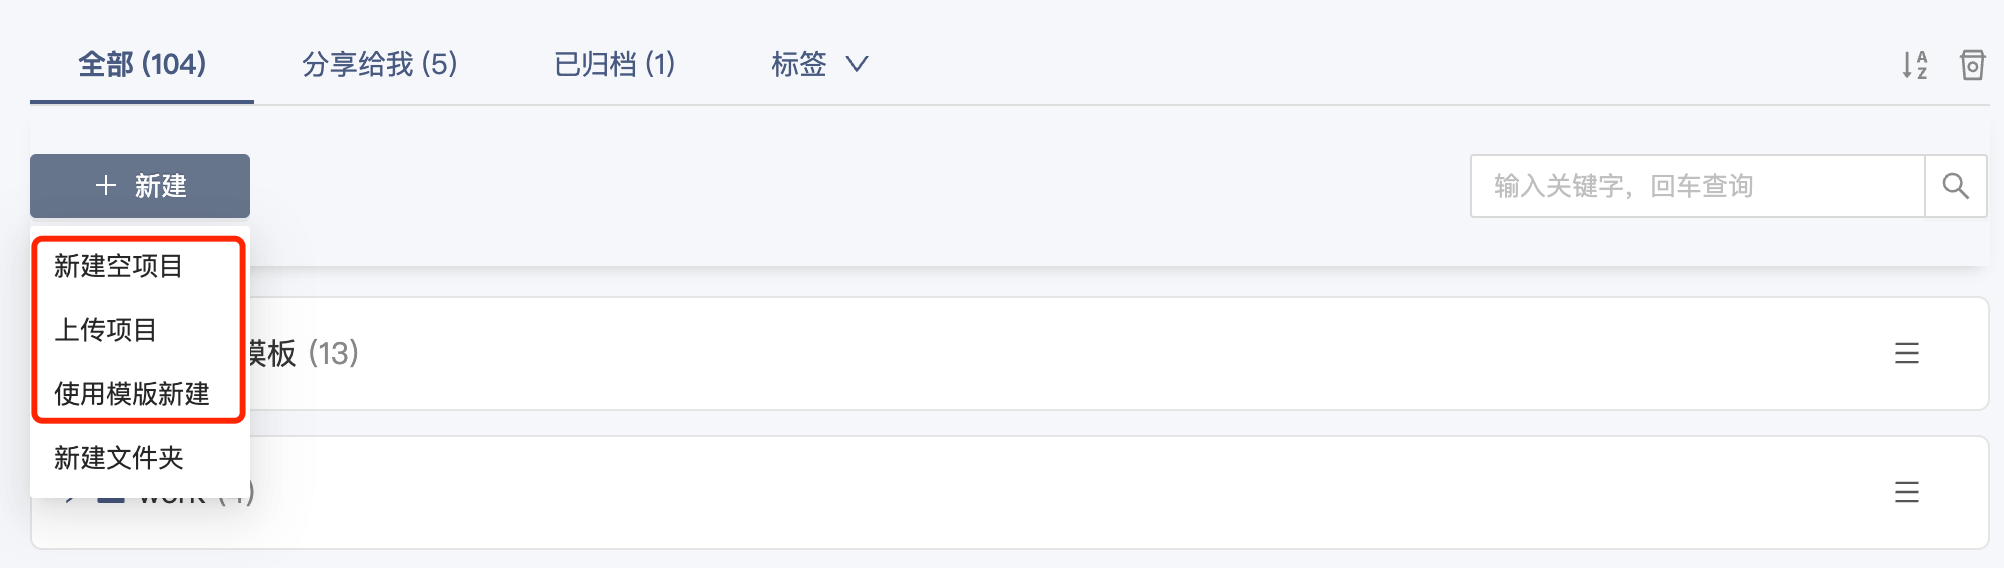
\includegraphics[width=\textwidth]{imgs/create.png}
\end{display}

\begin{itemize}
\item 创建空项目
\item 上传项目,支持上传 zip 文件
\item 通过模板创建项目
\end{itemize}
\end{frame}


\begin{frame}{\texpage 编辑器}
\texpage 编辑器分为 3 个部分,可以通过拖拽边框
或点击边框中间的按钮,调整每个部分的宽度。

\begin{display}
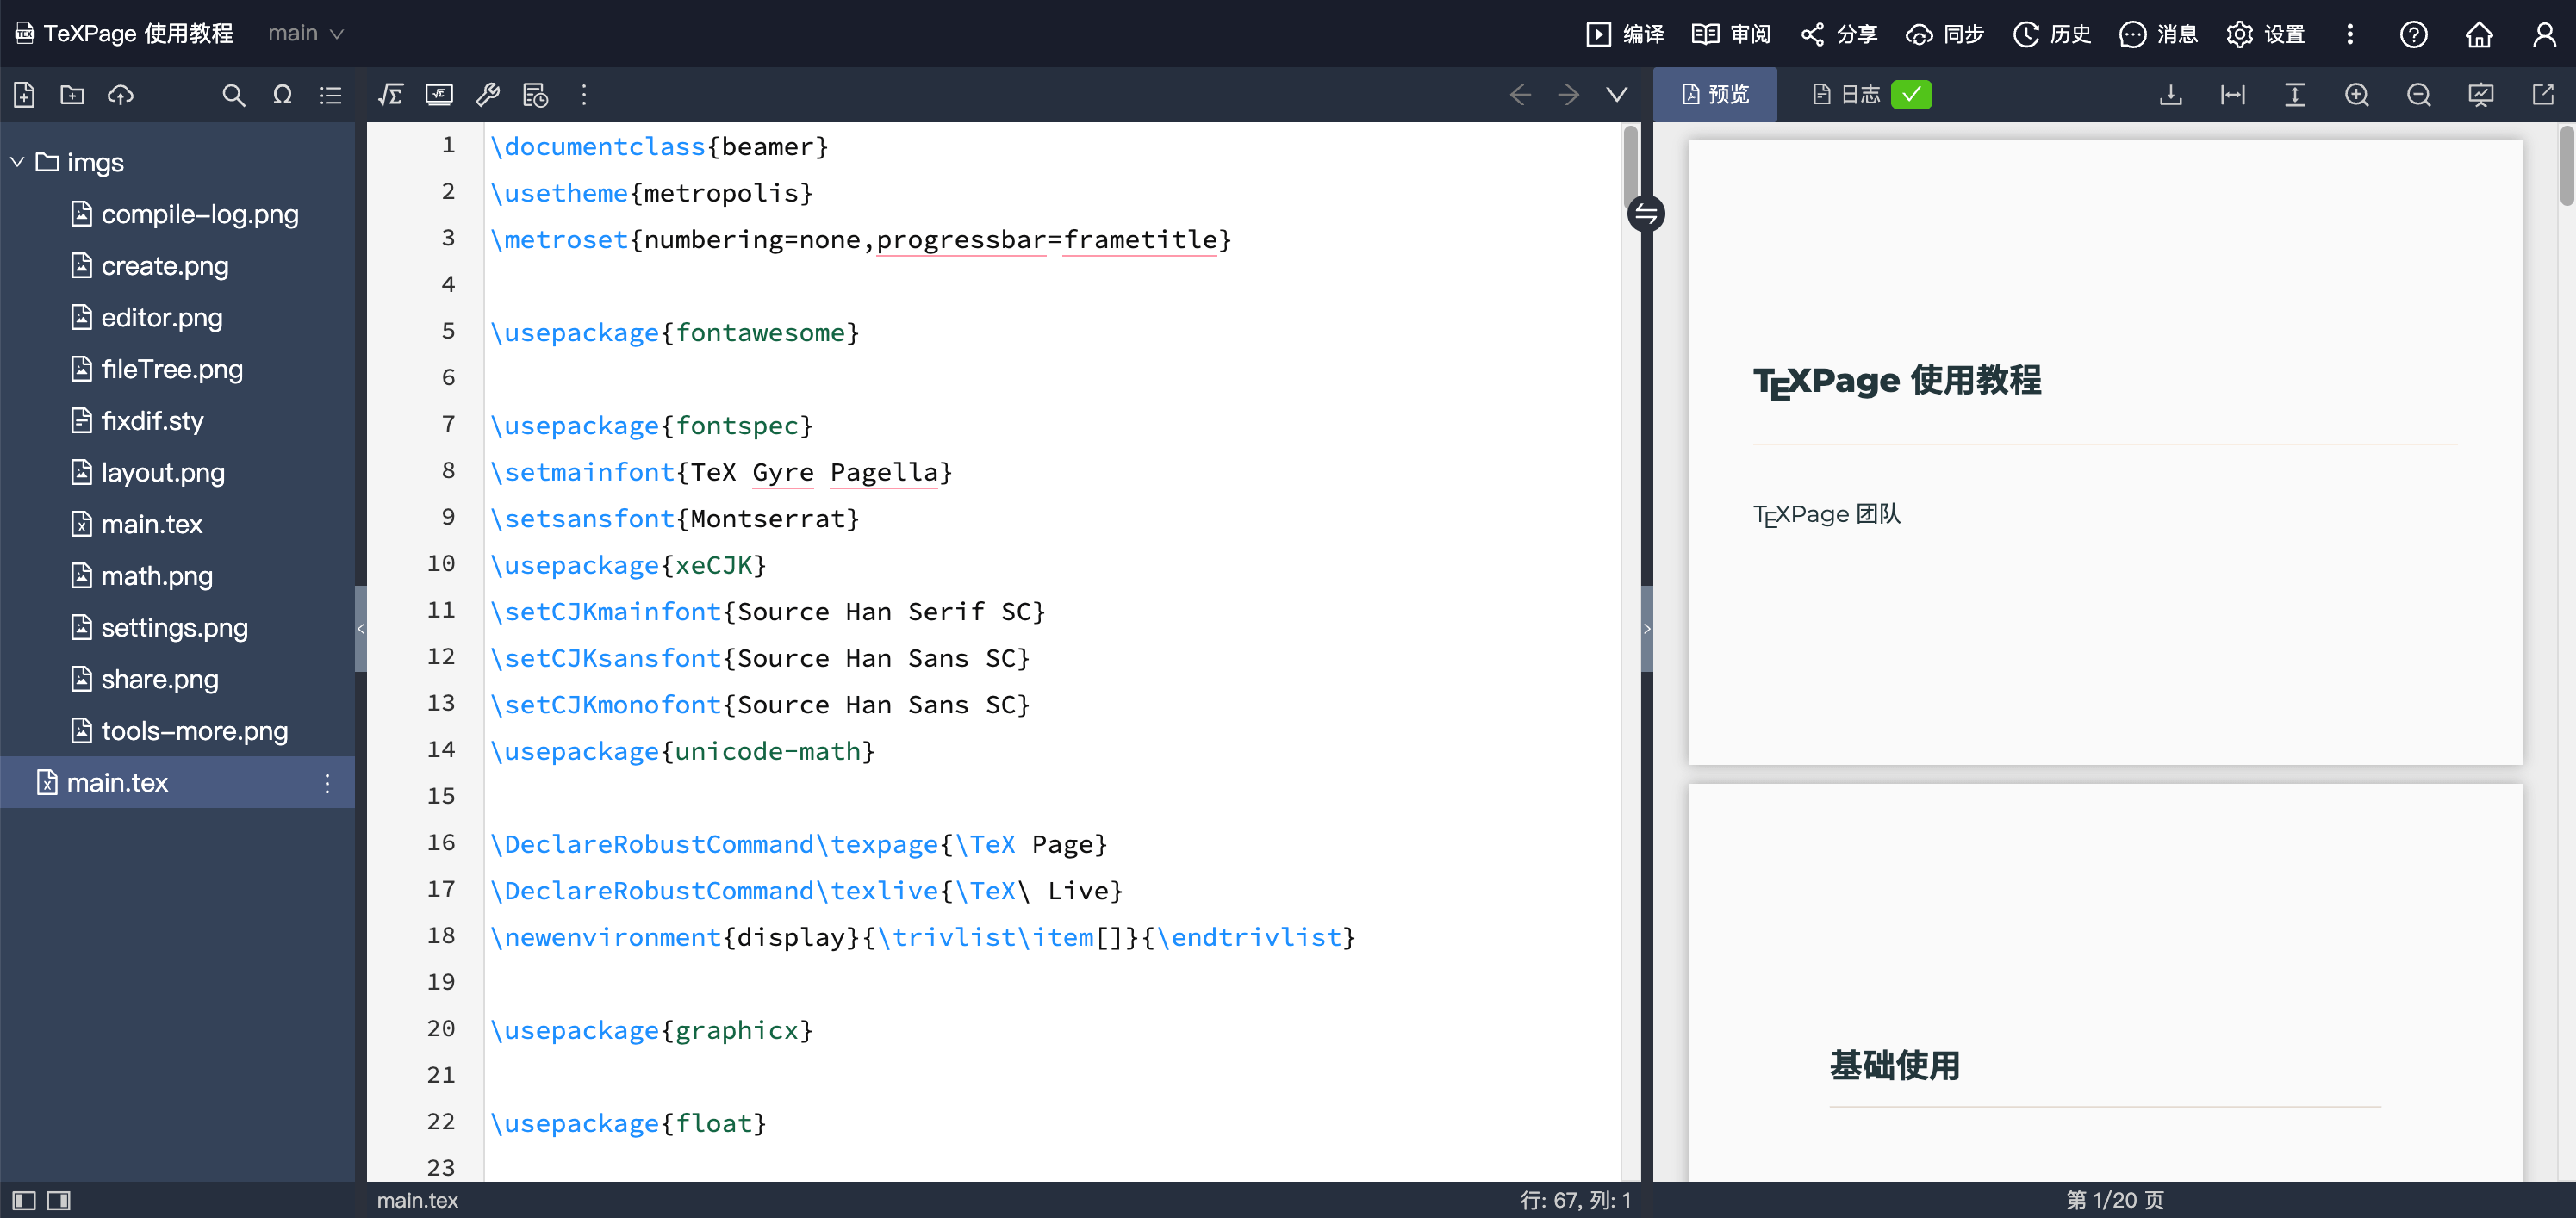
\includegraphics[width=\textwidth]{imgs/layout.png}
\end{display}

文件管理\hspace{\stretch{1}}
\LaTeX 编辑器\hspace{\stretch{2}}
PDF 预览\hspace*{\stretch{1}}

\end{frame}


\begin{frame}{编写 \LaTeX 代码}
\texpage 开发了体验友好的 \LaTeX 编辑器,支持代码高亮,代码自动补全等常见功能。在编辑区域直接输入 \LaTeX 代码即可。

\begin{display}
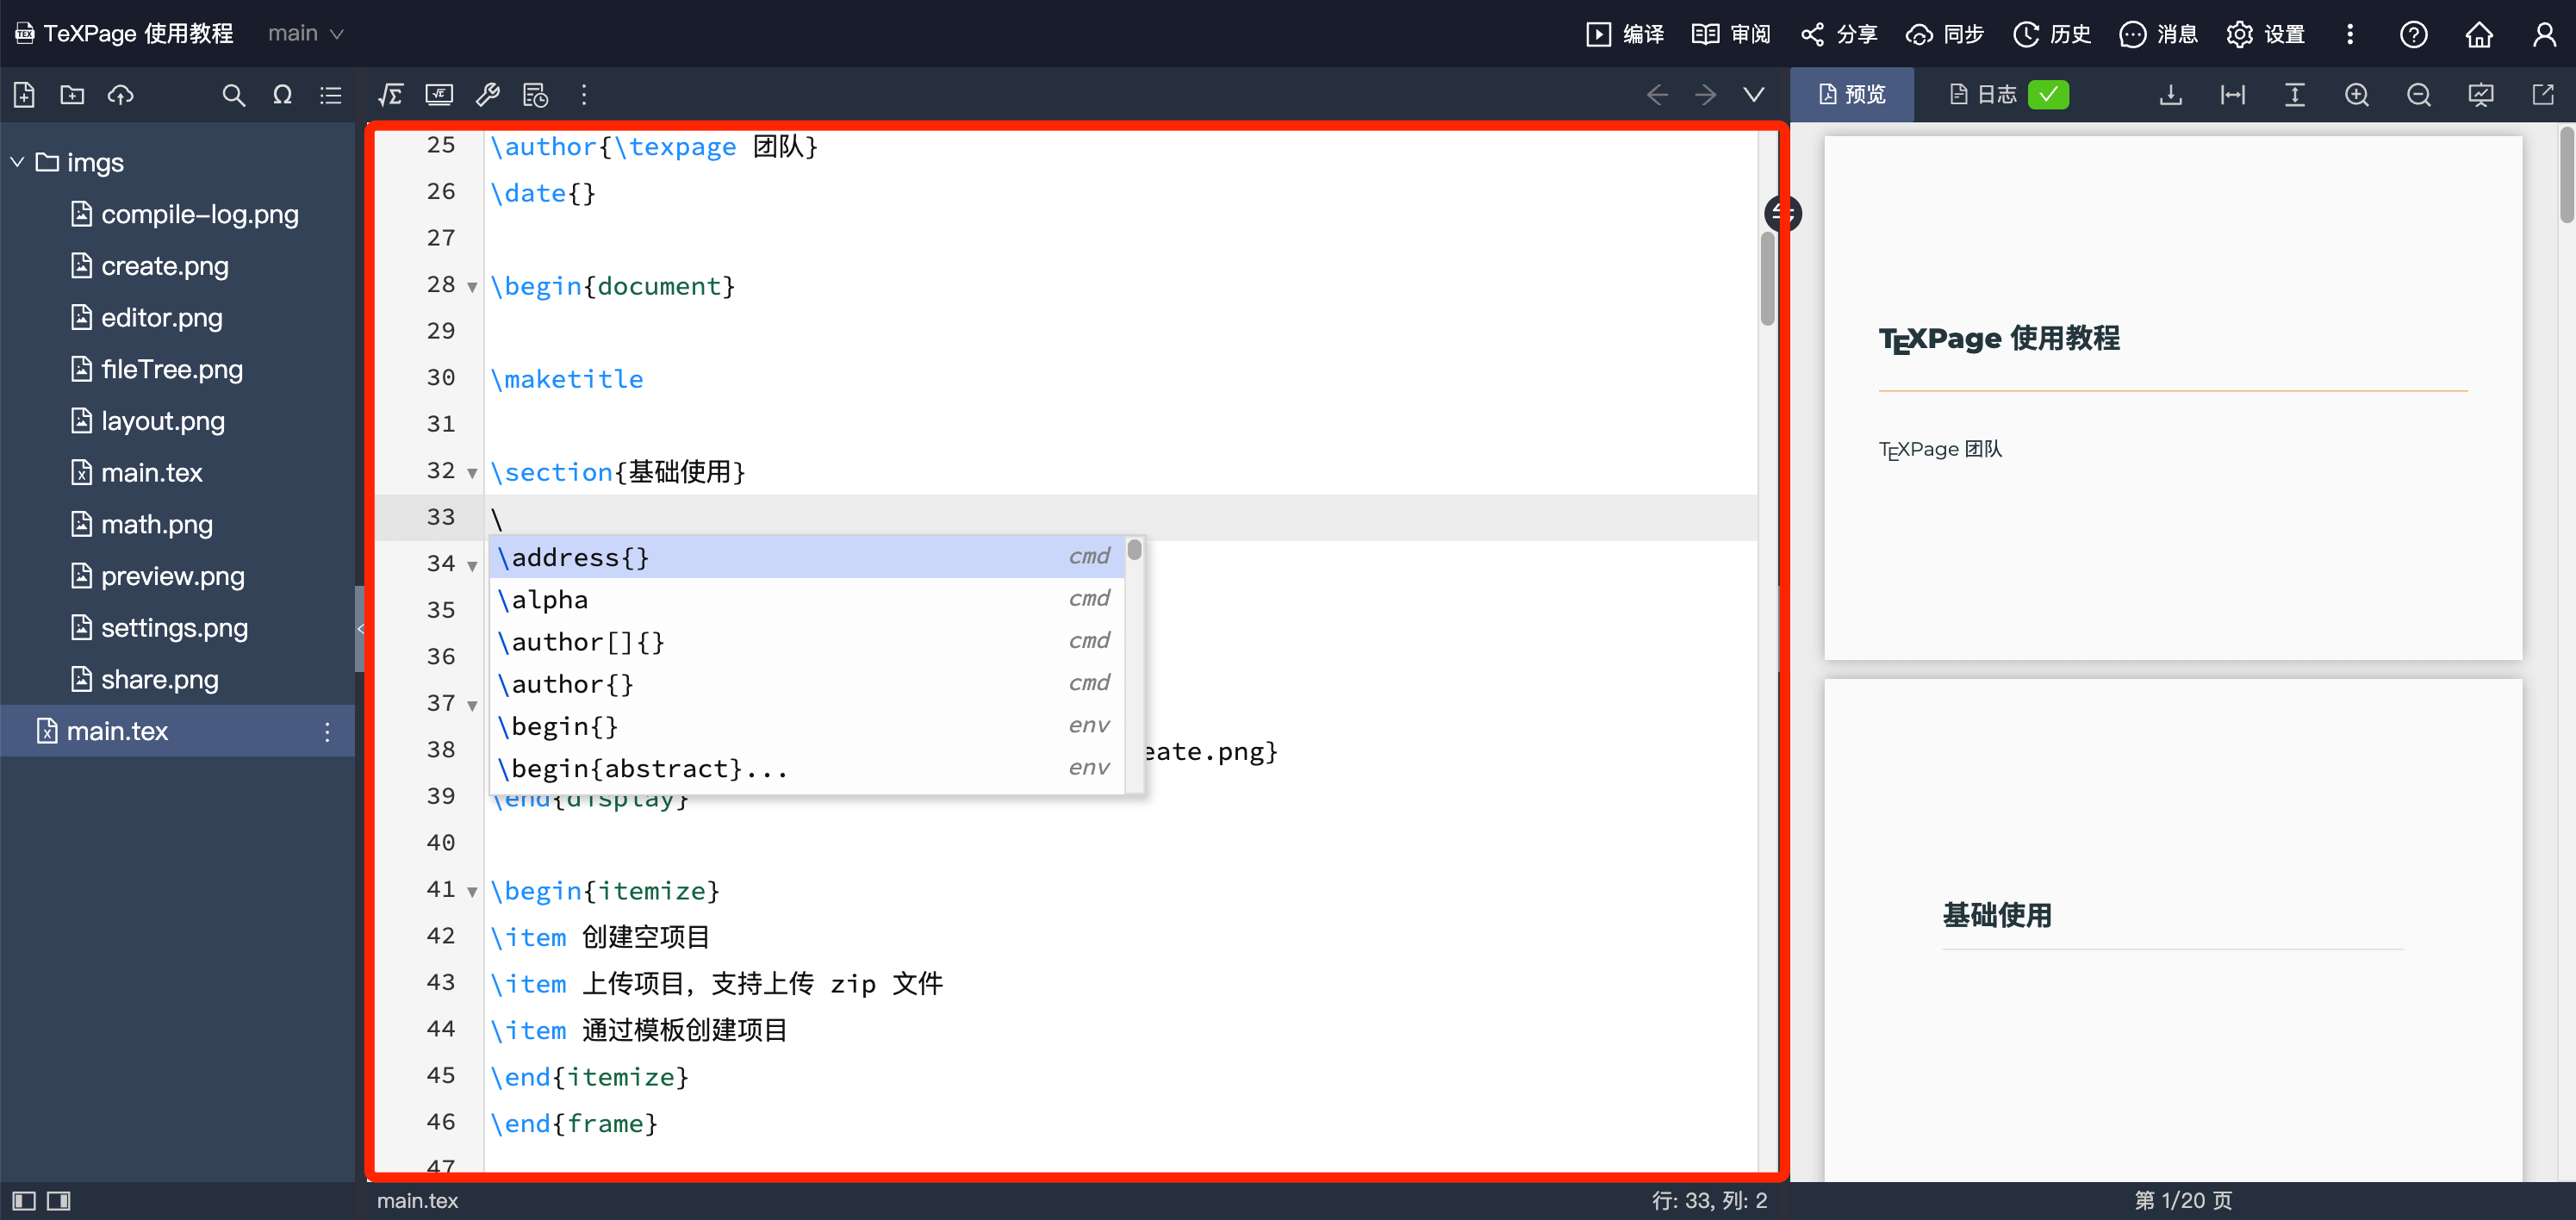
\includegraphics[width=\textwidth]{imgs/editor.png}
\end{display}
\end{frame}


\begin{frame}{编写 \LaTeX 代码}
\texpage 编辑器主要产品特性:

\begin{itemize}
\item \LaTeX 语法高亮
\item 代码 ↔ PDF 双向自动跳转:\textbf{双击}对应位置
\item \LaTeX 代码自动补全,自动补全常见命令、label 和 bib
\item bib 高级搜索,按照关键词搜索 bib 文件
\item 英文拼写检查
\item 括号自动补全
\item 文件大纲
\item 常用符号选择器
\end{itemize}
\end{frame}


\begin{frame}{编译 \LaTeX 文件}
\texpage 编译服务主要产品特性:
\begin{itemize}
    \item 在线编译 LaTeX 文档,用户无需安装 \TeX 发行版
    \item 自动处理 LaTeX 编译流程
    \item 自动处理编译缓存,提升编译速度
    \item 完善的编译环境,满足各种场景的编译需求
\end{itemize}

\end{frame}


\begin{frame}{编译 \LaTeX 文件\hfill ——编译前}
\begin{itemize}
\item 检查 \LaTeX 项目主文件设置是否正确,
在顶部操作栏设置里查看或修改主文件配置
\item 确定编译器以及 \texlive 版本,同样在设置里配置
\end{itemize}

\begin{display}
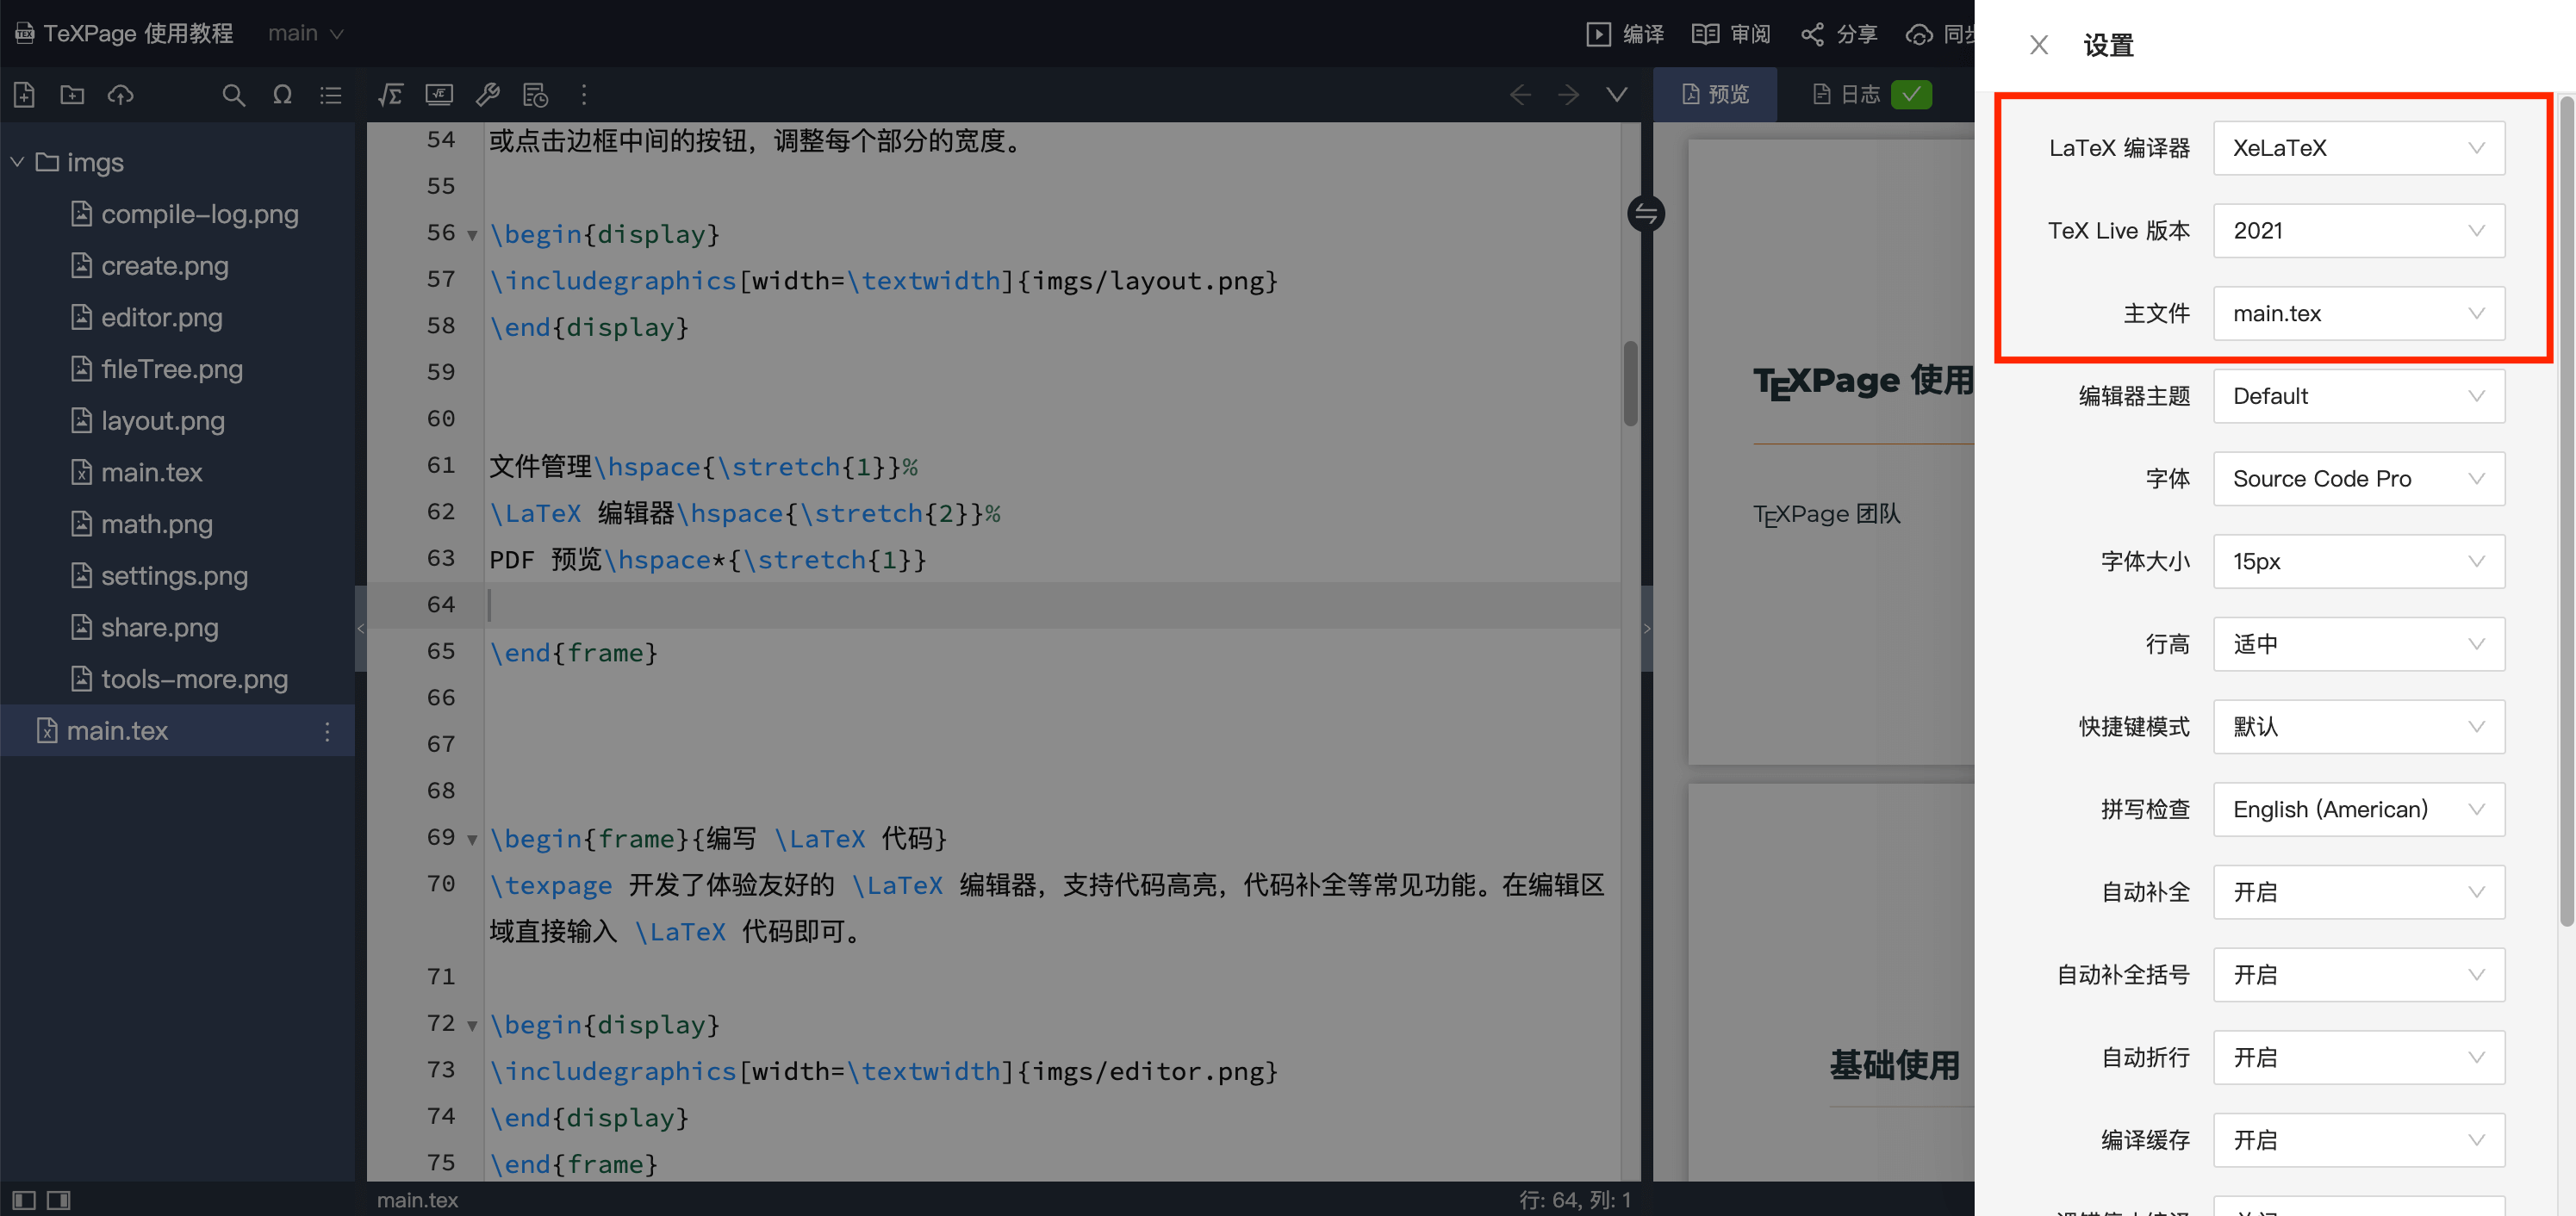
\includegraphics[width=\textwidth]{imgs/settings.png}
\end{display}
\end{frame}


\begin{frame}{编译 \LaTeX 文件\hfill ——编译}
\begin{itemize}
\item 点击顶部操作栏的「编译」按钮
\item Windows 下可使用 Ctrl + S 或 Ctrl + Enter 快捷键
\item macOS 下可使用 Command + S 或 Command + Enter 快捷键
\end{itemize}

\begin{display}

\includegraphics[width=\textwidth]{imgs/compile-btn.png}
\end{display}
\end{frame}


\begin{frame}{编译 \LaTeX 文件\hfill ——查看 PDF 和日志}
最右侧区域是 PDF 预览和编译日志区域。

在预览顶部日志标签右侧会提示编译错误和警告数量:
\begin{itemize}
\item \textbf{\color{red}错误}用红色标识
\item \textbf{\color{orange}警告}用橙色标识
\item \textbf{\color{green!80!black}编译成功}(无报错/警告)用绿色标识
\end{itemize}

\end{frame}


\begin{frame}{编译 \LaTeX 文件\hfill ——PDF 预览}
\begin{itemize}
\item 支持放大、缩小、铺满宽度和铺满高度四种缩放操作
\item 支持全屏放映模式和全屏预览模式
\item 双击 PDF 会将编辑器跳转到对应的 \LaTeX 代码所在位置
\end{itemize}

\begin{display}
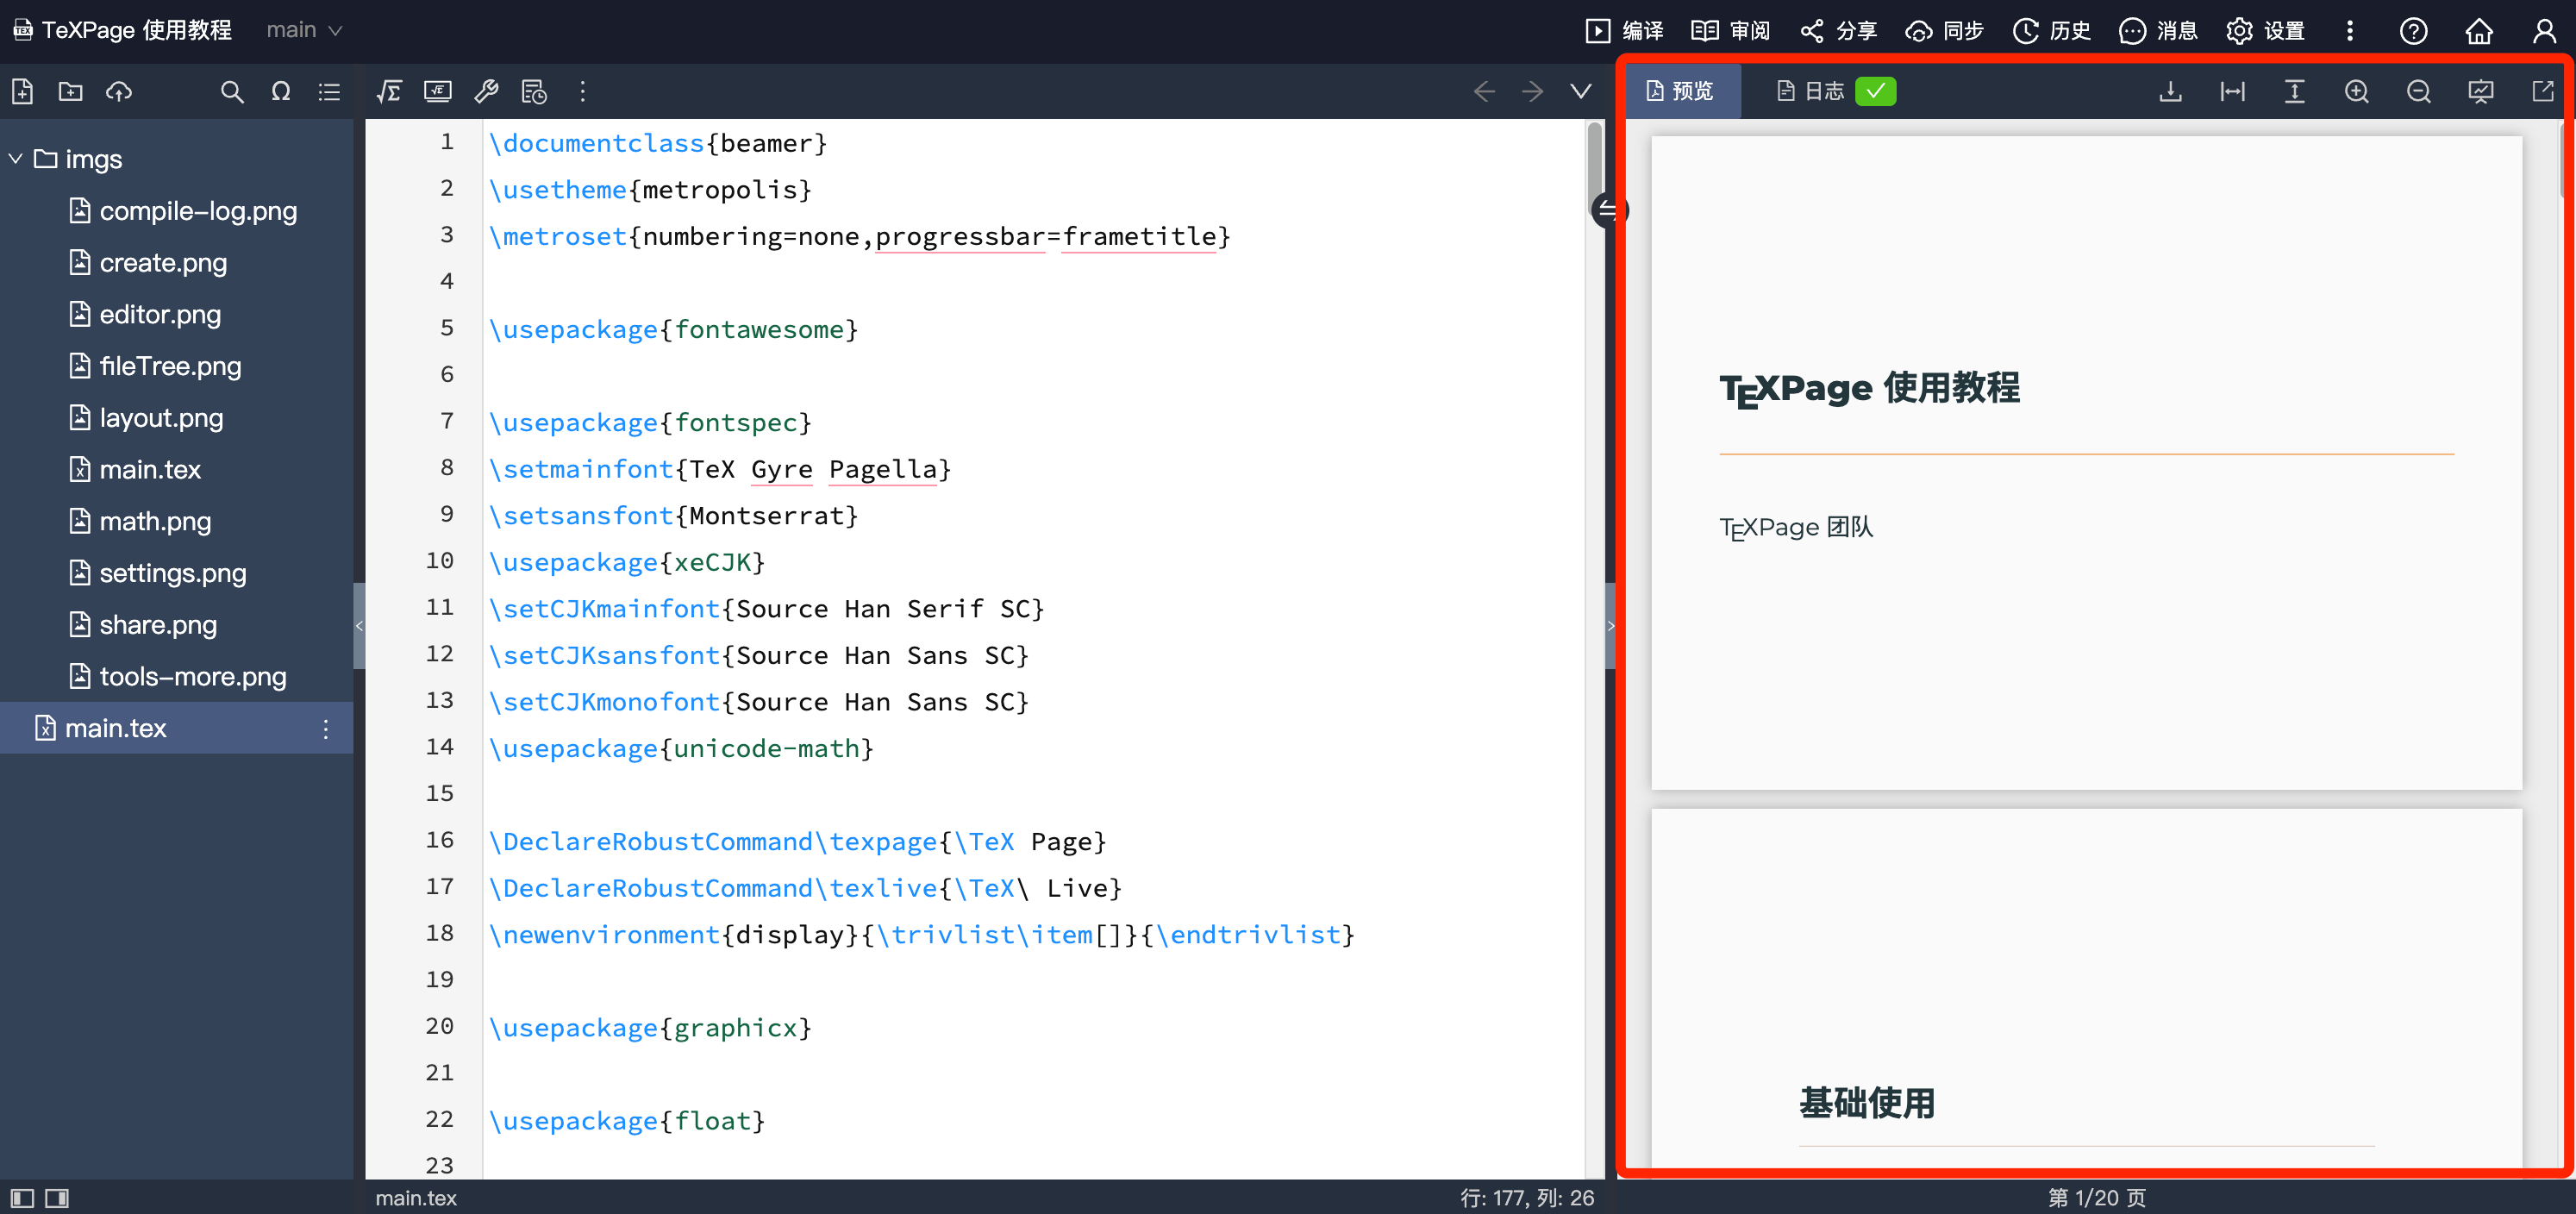
\includegraphics[width=\textwidth]{imgs/preview.png}
\end{display}

\end{frame}


\begin{frame}{编译 \LaTeX 文件\hfill ——编译日志}
\begin{itemize}
\item 分类显示\textbf{\color{red}错误}和\textbf{\color{orange}警告}
\item 点击\textbf{\color{red}错误}信息后跳转到对应的错误代码处
\item 在日志区域底部能够展开查看原始日志
\item 需要清空编译缓存时,在原始日志右侧点击「清空编译缓存」
\end{itemize}

\begin{display}

\includegraphics[width=\textwidth]{imgs/compile-log.png}
\end{display}

\end{frame}


\begin{frame}{管理 \LaTeX 项目}
左侧部分是项目文件管理部分,项目文件以目录树的形式展示。
文件操作区域在目录树顶部和每个文件名称的最右侧。

支持新建文件/文件夹、重命名文件/文件夹、
上传文件和删除文件/文件夹等操作。

\begin{center}
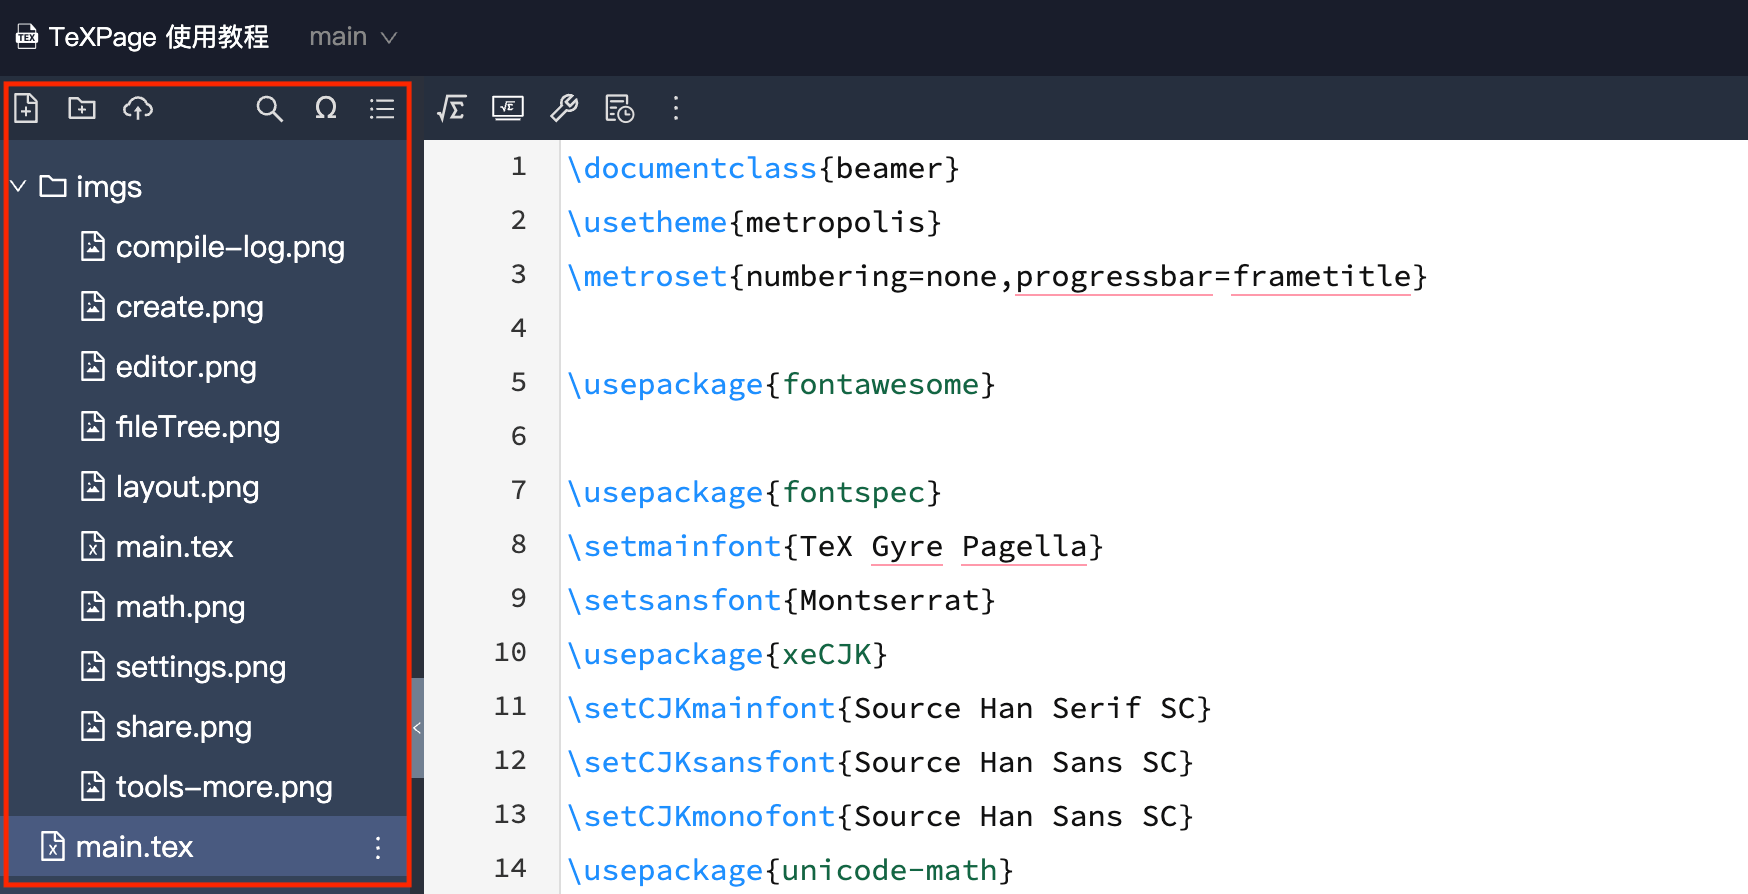
\includegraphics[width=0.9\textwidth]{imgs/fileTree.png}
\end{center}
\end{frame}


\section{在线协作}

\begin{frame}{分享项目}
点击顶部操作栏的「分享」按钮,会弹出分享项目对话框,将分享链接发送协作者,协作者点击链接后会自动加入项目。

\begin{center}
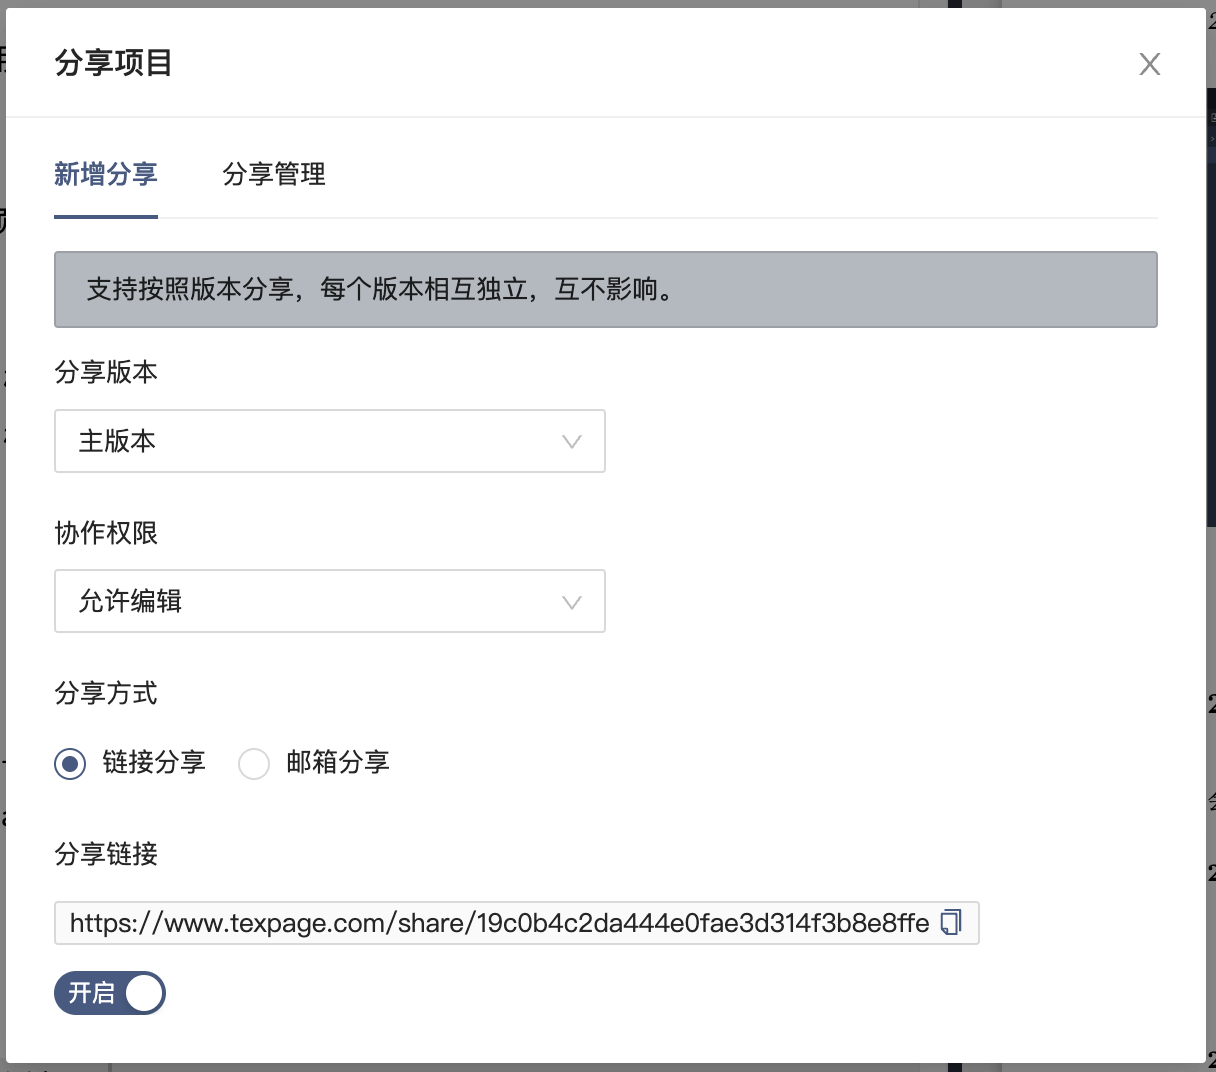
\includegraphics[width=.7\textwidth]{imgs/share.png}
\end{center}

\end{frame}


\begin{frame}{审阅功能}
审阅功能包括:
\begin{itemize}
\item 批注:所有用户都可使用批注功能
\item 追踪变更:开启后会记录每一次编辑,可选择接受或拒绝编辑记录
\end{itemize}
具体使用教程详见:\href{https://www.texpage.com/docs/features/texpage-review/}{\textbf{审阅功能使用教程{}>>}}
\end{frame}

\section{版本管理}
\begin{frame}{版本管理}
\texpage 中的 \LaTeX 项目可以创建多个版本,默认版本名称是 main。

版本管理的应用场景:
\begin{itemize}
    \item 多人协作时,新建独立版本给协作者,不同版本互不影响
    \item 在重要节点存档 \LaTeX 项目版本,创建版本时审阅记录会自动同步到新版本
    \item 比对多个版本的差异,生成修订版本的 PDF
\end{itemize}

\begin{display}
    \centering
    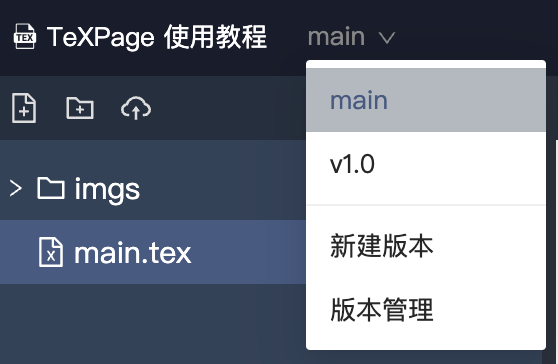
\includegraphics[width=.35\textwidth]{imgs/version-entry.png}
\end{display}
\end{frame}

\section{好用的工具}

\begin{frame}{公式编辑器}
\begin{center}
    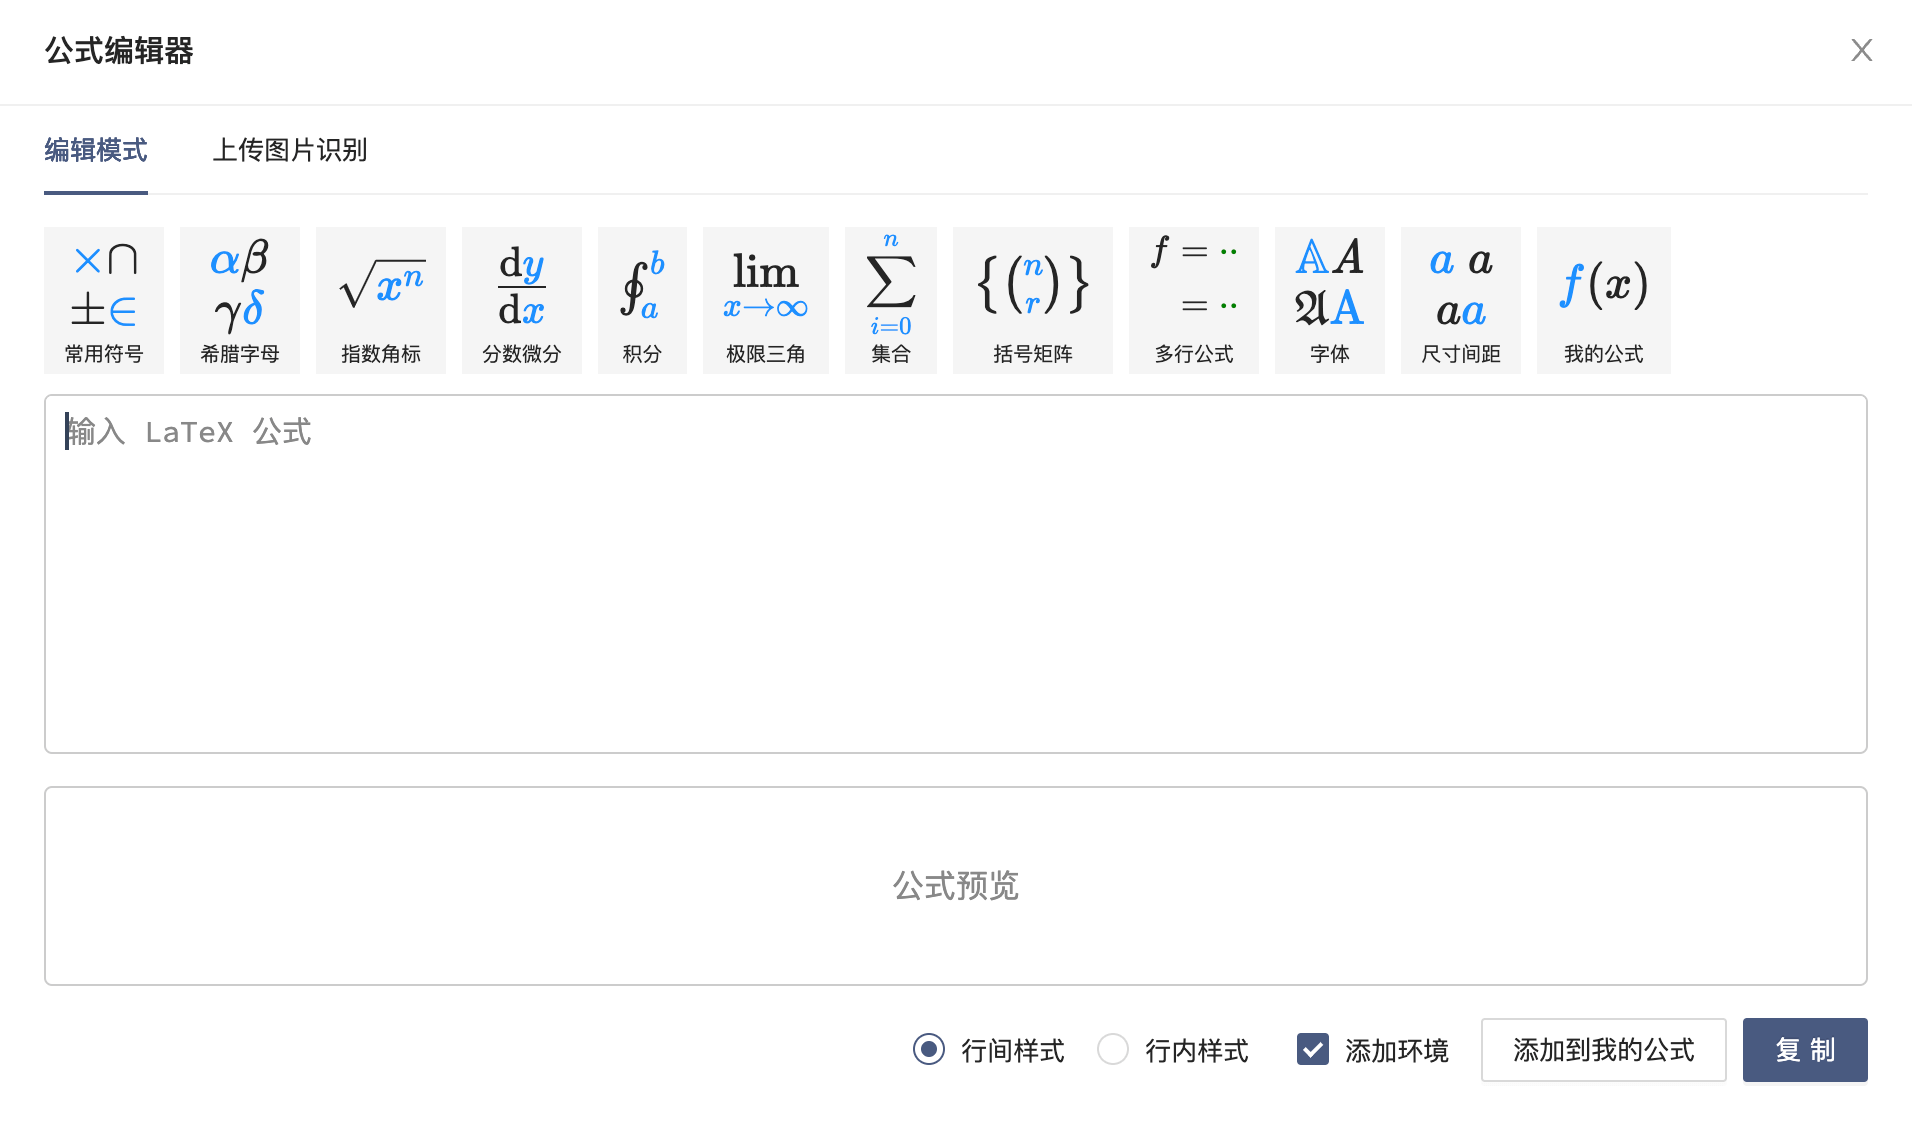
\includegraphics[width=\textwidth]{imgs/math.png}
\end{center}
\end{frame}

\begin{frame}{表格设计器}
\begin{center}
    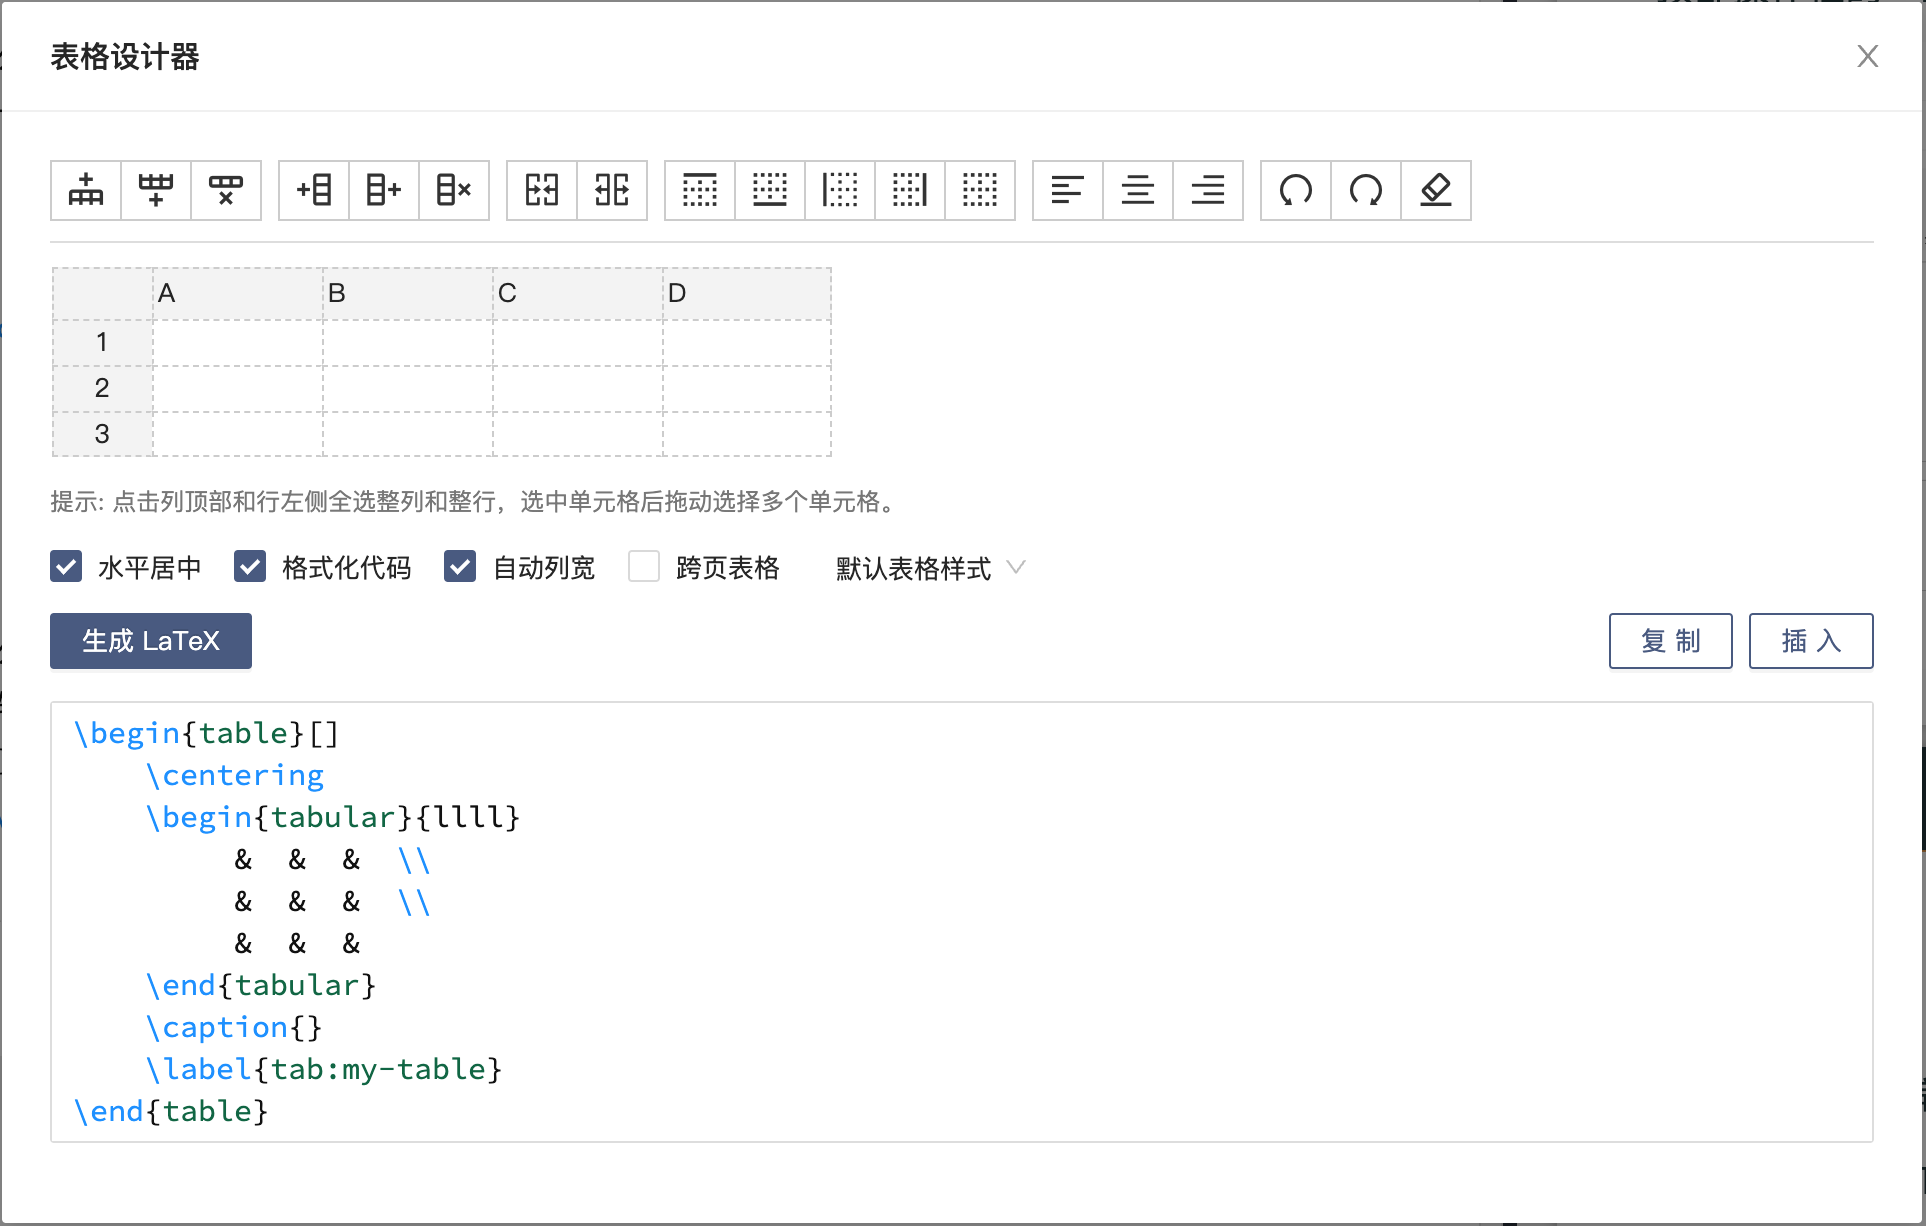
\includegraphics[width=\textwidth]{imgs/table-generator.png}
\end{center}
\end{frame}

\begin{frame}[standout]
\begin{center}
\Large 更多请见:
\href{https://www.texpage.com/docs/}{\textbf{\texpage 文档中心{}>>}}
\end{center}
\end{frame}

\end{document}
